\chapter{Producción}

\subsection{Subir Spring a heroku}

Para poner en producción el proyecto se necesitan seguir los siguientes pasos.

\subsection{Github}
\begin{itemize}
    \item Una vez hecho los cambios del sistema o darle mantenimiento, se tiene que ejecutar en terminal los siguientes comandos: 
    git add .
    git commit -m "algún comentario acerca de los cambios"
    git pull
    git push origin master
    \item Una vez hecho esto, se tendrán la actualización del proyecto en github.
    \item Después de esto, se necesita ir a heroku, donde se harán los siguientes paso 
\end{itemize}
Una vez que este actualizado el proyecto en github, se tiene que ir a heroku, donde se seguiran los siguientes pasos para subir el servidor de api rest.
\subsection{Heroku}
\begin{itemize}
    \item Se tiene que dirigir al navegador y entrar a la página principal de heroku.
    \item Se tiene que contactar con el administrador quien le dará permisos para poder hacer deploy de los cambios en el servidor de producción.
    \item Al iniciar sesión en heroku, se verá la pantalla de la figura 7.1.
    \item Después de esto, daremos click en el botón que se indica en la figura 7.2.
    \item Este botón nos abrirá la pantalla de la figura 7.3.
    \item Nos deslizaremos hacía abajo, hasta ver la pantalla de la figura 7.4.
    \item Veremos una sección que se llama Manual Deploy, en está se indica un botón que tiene por titulo Deploy Branch figura 7.5.
    \item Esperaremos hasta que se termine de ejecutar el deploy con el mensaje de Build Succes figura 7.6.
    \item Una vez hecho estos pasos, se tendrá el servidor de API Rest para producción.
\end{itemize}



\begin{figure}[!h]
	\centering
	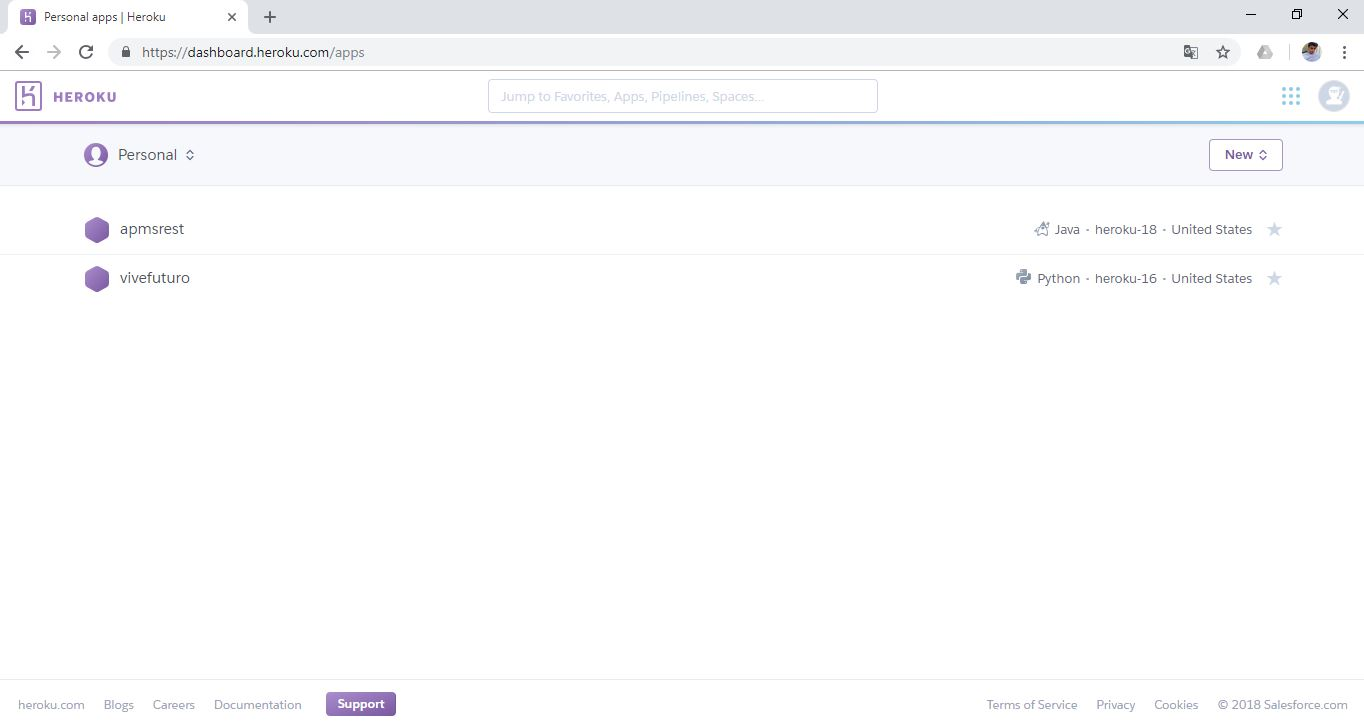
\includegraphics[width=0.7\linewidth]{images/tecnologias/heroku.JPG}
	\caption{Entorno de producción Heroku.}
\end{figure}


\begin{figure}[!h]
	\centering
	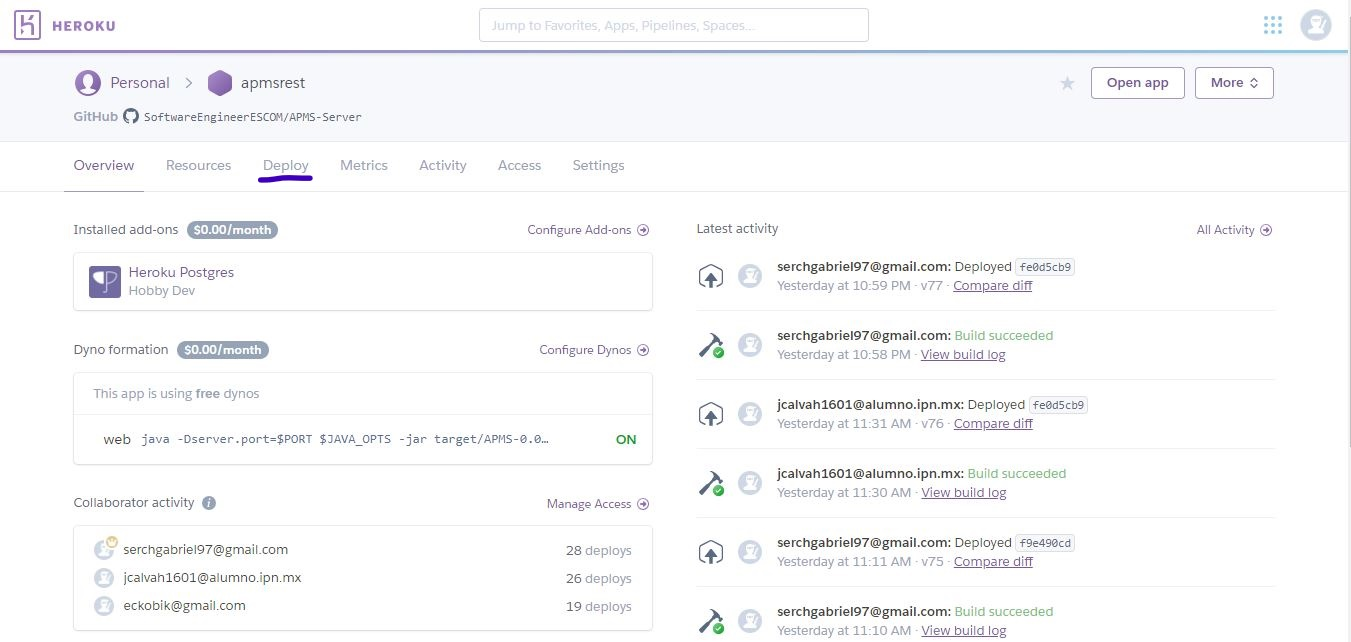
\includegraphics[width=0.7\linewidth]{images/tecnologias/heroku2p.png}
	\caption{Botón para ejecutar el sistema.}
\end{figure}


\begin{figure}[!h]
	\centering
	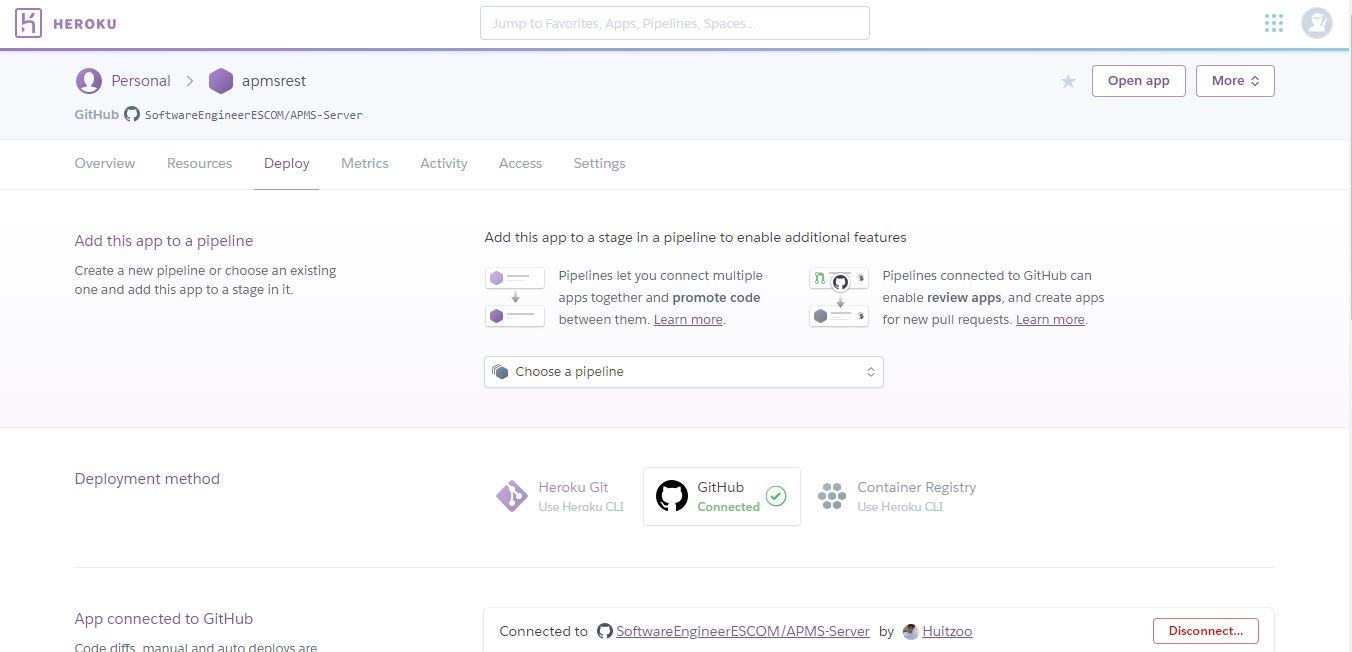
\includegraphics[width=0.7\linewidth]{images/tecnologias/heroku3.JPG}
\end{figure}


\begin{figure}[!h]
	\centering
	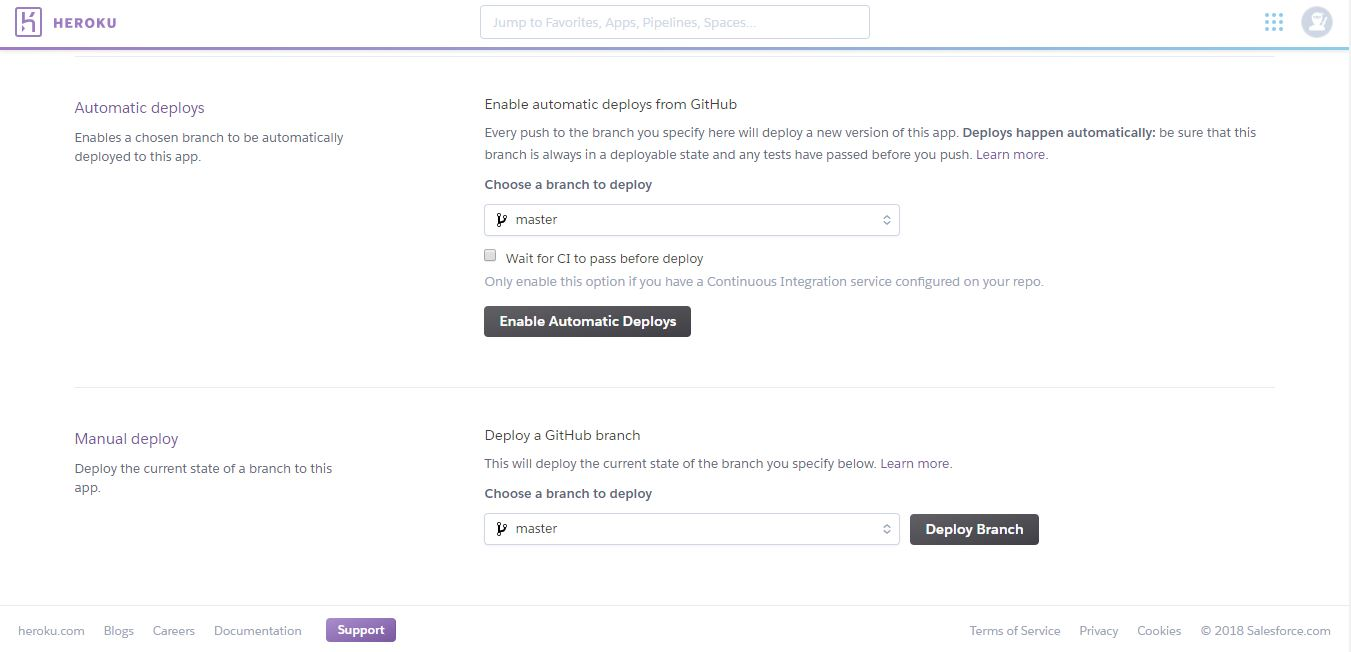
\includegraphics[width=0.7\linewidth]{images/tecnologias/heroku4.JPG}
\end{figure}

\begin{figure}[!h]
	\centering
	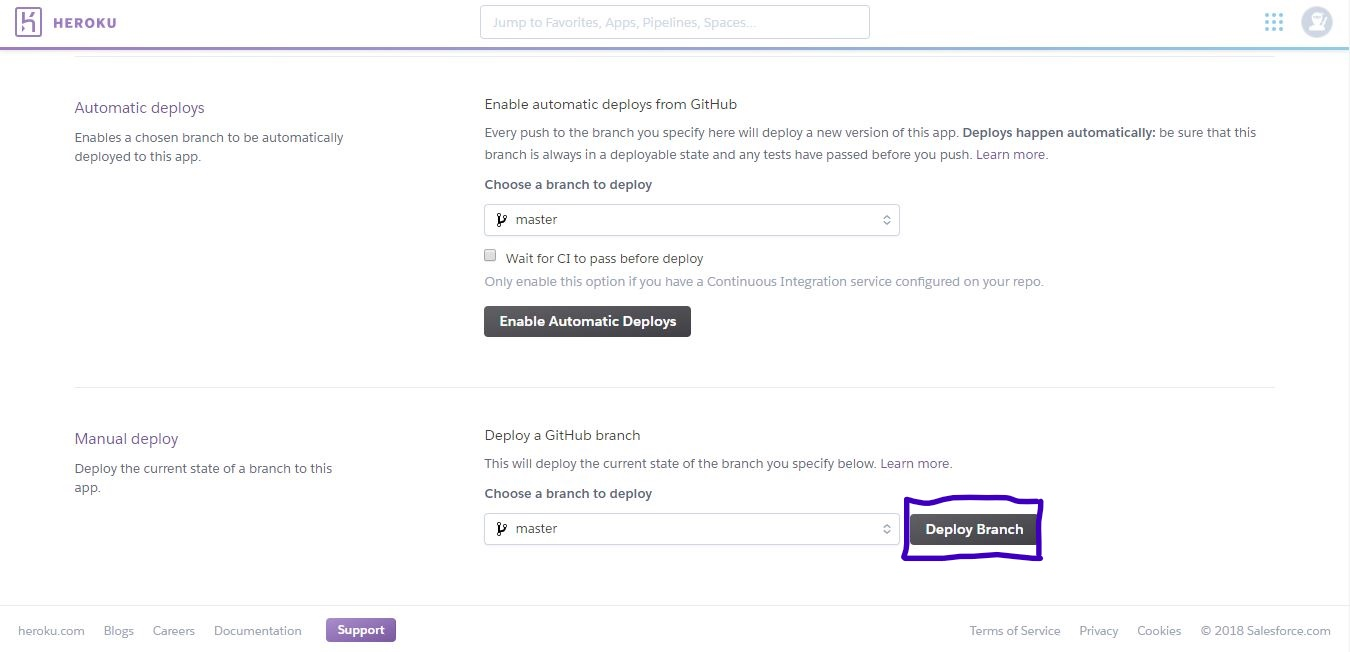
\includegraphics[width=0.7\linewidth]{images/tecnologias/heroku4p.JPG}
\end{figure}

\begin{figure}[!h]
	\centering
	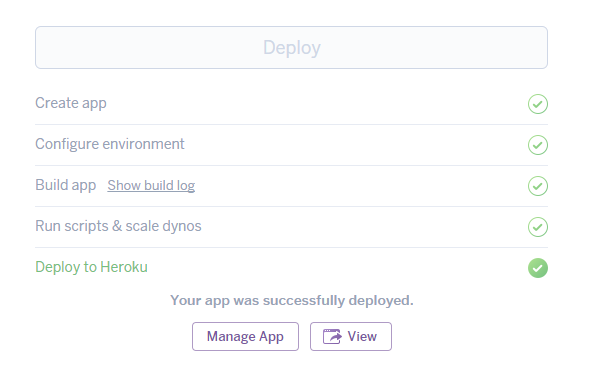
\includegraphics[width=0.7\linewidth]{images/tecnologias/heroku6.PNG}
	\caption{Mensaje de éxito al terminar de subir el proyecto en heroku.}
\end{figure}

\subsection{Angular}
